\documentclass[runningheads]{llncs}

\usepackage{amsmath, amssymb}
\usepackage{tikz}

\usetikzlibrary{shapes, arrows}

\newcommand{\east}{{\ensuremath \to}}
\newcommand{\se}{{\ensuremath \searrow}}

\DeclareMathOperator*{\argmin}{arg\,min}

\title{Towards the Algorithmic Molecular Self-Assembly of Fractals by Cotranscriptional Folding\thanks{This work is in part supported by JST Program to Disseminate Tenure Tracking System, MEXT, Japan, No.~6F36 and by JSPS KAKENHI Grant-in-Aid for Young Scientists (A) No.~16H05854 to S.~S.}}
\titlerunning{Algorithmic Self-Assembly of Fractals by Cotranscriptional Folding}
\author{
Yusei Masuda \and 
Shinnosuke Seki\thanks{Corresponding author} \and 
Yuki Ubukata
}
\institute{
Department of Computer and Network Engineering, 
The University of Electro-Communications, 
1-5-1, Chofugaoka, Chofu, Tokyo, 1828585, Japan 
\email{s.seki@uec.ac.jp}
}

\begin{document}

\maketitle

\begin{abstract}

\end{abstract}

%--------------------------------------------------------------------------------------------------------
	\section{Introduction}
%--------------------------------------------------------------------------------------------------------

%--------------------------------------------------------------------------------------------------------
	\section{Preliminaries}
%--------------------------------------------------------------------------------------------------------

Let $\Sigma$ be a set of types of abstract molecules, or \textit{beads}, and $\Sigma^*$ be the set of finite sequences of beads. 
A bead of type $a \in \Sigma$ is called an $a$-bead. 
Let $w = b_1 b_2\cdots b_n \in \Sigma^*$ be a string of length $n$ for some integer $n$ and bead types $b_1, \ldots, b_n \in \Sigma$.
The \textit{length} of $w$ is denoted by $|w|$, that is, $|w| = n$. 
For two indices $i,j$ with $1\leq i \leq j \leq n$, we let $w[i..j]$ refer to the subsequence $b_i b_{i+1} \cdots b_{j-1} b_{j}$; if $i=j$, then we simplify $w[i..i]$ as $w[i]$.
For $k \ge 1$, $w[1..k]$ is called a \textit{prefix} of $w$. 

Oritatami systems fold their transcript, a sequence of beads, over the triangular grid graph $\mathbb{T} = (V, E)$ as suggested in Fig.~\ref{fig:glider} cotranscriptionally based on hydrogen-bond-based interactions (\textit{h-interactions} for short) which the rule set of the system allow for between adjacent beads of particular types. 
A directed path $P = p_1 p_2 \cdots p_n$ in $\mathbb{T}$ is a sequence of \textit{pairwise-distinct} points $p_1, p_2, \ldots, p_n \in V$ such that $\{p_i, p_{i+1}\} \in E$ for all $1 \leq i < n$.
Its $i$-th point is referred to as $P[i]$. 
A \textit{rule set} $\mathcal{H} \subseteq \Sigma \times \Sigma$ is a symmetric relation over the set of pairs of bead types, that is, for all bead types $a, b \in \Sigma$, $(a, b) \in \mathcal{H}$ implies $(b, a) \in \mathcal{H}$. 

A \textit{conformation} $C$ is a triple $(P, w, H)$ of a directed path $P$ in $\mathbb{T}$, $w \in \Sigma^*$ of the same length as $P$, and a set of h-interactions $H \subseteq \{\{i,j\} \mid 1 \leq i, i+2 \leq j, \{P[i], P[j]\} \in E\}$.
This is to be interpreted as the sequence $w$ being folded in such a manner that its $i$-th bead $w[i]$ is placed on the $i$-th point $P[i]$ along the path and there is an h-interaction between the $i$-th and $j$-th beads if and only if $\{i, j\} \in H$. 
The condition $i+2 \leq j$ represents the topological restriction that two consecutive beads along the path cannot form an h-interaction between them.
Let $\mathcal{H}$ be a rule set. 
An h-interaction $(i, j) \in H$ is \textit{valid with respect to $\mathcal{H}$}, or simply \textit{$\mathcal{H}$-valid}, if $(w[i], w[j]) \in \mathcal{H}$. 
This conformation $C$ is $\mathcal{H}$-valid if all of its h-interactions are $\mathcal{H}$-valid. 
%For an integer $\alpha \ge 1$, $C$ is \textit{of arity $\alpha$} if the maximum number of h-interactions per bead is $\alpha$, that is, if for any $k \ge 1$, $|\{i \mid (i, k) \in H)\}| + |\{j \mid (k, j) \in H\}| \le \alpha$ and this inequality holds as an equation of some $k$. 
For an integer $\alpha \ge 1$, $C$ is \textit{of arity $\alpha$} if $C$ contains a bead that forms $\alpha$ h-interactions and no bead of $C$ forms more. 
By $\mathcal{C}_{\le \alpha}$, we denote the set of all conformations of arity at most $\alpha$.

Oritatami systems grow conformations by elongating them under their own rule set. 
Given a rule set $\mathcal{H}$ and an $\mathcal{H}$-valid finite conformation $C_1 = (P, w, H)$, 
we say that another conformation $C_2$ is an \textit{elongation of} $C_1$ \textit{by a bead} $b \in \Sigma$, written as $C_1 \xrightarrow{\mathcal{H}}_b C_2$, if $C_2 = (Pp, wb, H \cup H')$ for some point $p$ not along the path $P$ and set of h-interactions $H' \subseteq \left\{ \{i, |w|+1\} \bigm| 1\leq i < |w|, \{P[i], p\} \in E, (w[i], b) \in \mathcal{H}\right\}$, which can be empty.
Note that $C_2$ is also $\mathcal{H}$-valid.
This operation is recursively extended to the elongation by a finite sequence of beads as: 
for any conformation $C$, $C \xrightarrow{\mathcal{H}}^*_\lambda C$; 
and for a finite sequence of beads $w \in \Sigma^*$ and a bead $b \in \Sigma$,
a conformation $C_1$ is elongated to a conformation $C_2$ by $wb$,
written as $C_1 \xrightarrow{\mathcal{H}}^*_{wb} C_2$, if there is a conformation $C'$ that satisfies
$C_1 \xrightarrow{\mathcal{H}}^*_w C'$ and $C' \xrightarrow{\mathcal{H}}_b C_2$.

A finite \textit{oritatami system} (OS) is a 5-tuple $\Xi = (\mathcal{H}, \alpha, \delta, \sigma,w)$, where 
$\mathcal{H}$ is a rule set,
$\alpha$ is an arity, 
$\delta \geq 1$ is a parameter called the \textit{delay}, 
$\sigma$ is an initial $\mathcal{H}$-valid conformation of arity $\alpha$ called the \textit{seed}, upon which its finite \textit{transcript} $w \in \Sigma^*$ is to be folded by stabilizing beads of $w$ one at a time so as to minimize energy collaboratively with the succeeding $\delta -1$ nascent beads. 
The energy of a conformation $C = (P, w, H)$, denoted by $\Delta G(C)$, is defined to be $-|H|;$ the more h-interactions a conformation has, the more stable it gets.
The set $\mathcal{F}(\Xi)$ of conformations \textit{foldable} by this system is recursively defined as: 
the seed $\sigma$ is in $\mathcal{F}(\Xi)$; and provided that an elongation $C_{i}$ of $\sigma$ by the prefix $w[1..i]$ be foldable (i.e., $C_0 = \sigma$), its further elongation $C_{i+1}$ by the next bead $w[i+1]$ is foldable if
\begin{equation}\label{eq:cotranscriptional_folding}
C_{i+1} \in \argmin_{
\substack{
C \in \mathcal{C}_{\le \alpha} s.t. \\
C_i \xrightarrow{\mathcal{H}}_{w[i+1]}C \\
}
}
\min \Big\{ \Delta G(C') \mid 
C \xrightarrow{\mathcal{H}}^*_{w[i+2...i+k]}C', k\le \delta, C' \in \mathcal{C}_{\le \alpha}
\Big\}.
\end{equation}
We say that the bead $w[i+1]$ and the h-interactions it forms are \textit{stabilized} according to $C_{i+1}$.
Note that an arity-$\alpha$ OS cannot fold any conformation of arity larger than $\alpha$.
The OS $\Xi$ is \textit{deterministic} if for all $i \ge 0$, there exists at most one $C_{i+1}$ that satisfies \eqref{eq:cotranscriptional_folding}. 

%--------------------------------------------------------------------------------------------------------
	\section{Folding the $n$-bit Heighway dragon}
%--------------------------------------------------------------------------------------------------------

We propose a generic design of deterministic cyclic OS that allows us to fold an arbitrary finite portion $P[j_1 .. j_2]$ of the slanted Heighway dragon. 
Independently of $j_1, j_2$, the design sets both delay and arity to 3 and employs 567 bead types with a fixed rule set $\mathcal{H}$ (some of the bead types might be saved but not easily due to the NP-hardness of minimizing the number of bead types \cite{HanKim2017}). 

One period is semantically divided into six parts (\textit{modules}) as $C F_v T C F_h T$, where %$C$ is called a \textit{counter module}, $F_v$ and $F_h$ are called a \textit{DFAO module}, and $T$ is called a \textit{turner module}. 
\begin{itemize}
\item $C$ is called a \textit{counter module}, which increments $i$ by 1 and propagates it; 
\item $F_v, F_h$ are called a \textit{DFAO module}, which computes $P[i]$ and interprets it properly as A(cute) or O(btuse); 
\item $T$ is called a \textit{turning module}, which makes a turn according to A/O. 
\end{itemize}
The first $C$ and $F_v$ modules fold into a vertical line segment, while the second $C$ and $F_h$ fold into the next line segment, which is guaranteed to be horizontal. 
The DFAO modules $F_v, F_h$ differ only in their way to interpret their intermediate outcome $P[i]$. 
The slanted dragon involves two types of left turn as well as two types of right turn: acute and obtuse. 
Observe that after (slanted) vertical line segments, the dragon turns left obtusely and right acutely, whereas after horizontal ones, it turns left acutely and right obtusely. 
Moreover, vertical and horizontal segments alternate on the dragon. 
Therefore, it suffices for $F_v$ and $F_h$ to compute $P[i] \in \{L, R\}$ in the same way and interpret it as $A$(cute)/$O$(btuse) in an opposite fashion as $F_v$ converts $L$ into $O$ and $R$ into $A$, while $F_h$ converts $L$ into $A$ and $R$ into $O$. 

\begin{figure}[tb]
\includegraphics[width=\linewidth]{Figs/seed_sample2.png}
\caption{The seed conformation for the 3-bit Heighway dragon encoding the initial count 100.}
\label{fig:seed}
\end{figure}

\paragraph{Seed conformation} encodes the initial count $j_1$ in its binary representation $b_n b_{n-1} \cdots b_1$ as
\begin{equation}\label{eq:turner_output}
	{\tt 499 \east 500 \east 501 \east 506 \east 507 \east \mbox{$\bigodot_{k = n}^1$} (w_{t, b_k} \east 350 \east 351 \east (356 \east 357 \east)^6)} 
%	& & \ {\tt 350 \east 351 \east 356 \east 357 \east 316 \east 317 \se}
\end{equation}
where ${\tt w_{t, 0} = 338 \east 339 \east 344 \east 345}$ and ${\tt w_{t, 1} = 346 \east 347 \east 348 \east 349}$. 

\paragraph{Counter module} is implemented essentially in the same manner as in \cite{GeMeScSe2016}. 
It takes the current count $i$ formatted as \eqref{eq:turner_output}, which is fed by the seed or by the previous turner module, and increments the count by 1 unless it is preceded by the seed, and outputs the resulting count in its binary representation $a_n a_{n-1} \cdots a_1$ in the following format:
\begin{equation}\label{eq:counter_output}{\tt 
	44 \east 45 \east 46 \east 75 \east 76 \east \mbox{$\bigodot_{k = n}^1$} (w_{c, a_k} \east (69 \east 70 \east)^5 75 \east 76 \east)
}\end{equation}
where ${\tt w_{c, 0} = 51 \east 52 \east 57 \east 58 \east 63 \east 64}$ and ${\tt w_{c, 1} = 59 \east 60 \east 61 \east 62 \east 63 \east 64}$. 

\paragraph{DFAO module}

\paragraph{Turner module}

%--------------------------------------------------------------------------------------------------------
	\bibliographystyle{plain}
	\bibliography{heighway_CIAA2018}
%--------------------------------------------------------------------------------------------------------

%--------------------------------------------------------------------------------------------------------
	\newpage
	\appendix
%--------------------------------------------------------------------------------------------------------

%--------------------------------------------------------------------------------------------------------
	\section{Module automaton}
%--------------------------------------------------------------------------------------------------------

\begin{figure}[h]
\centering
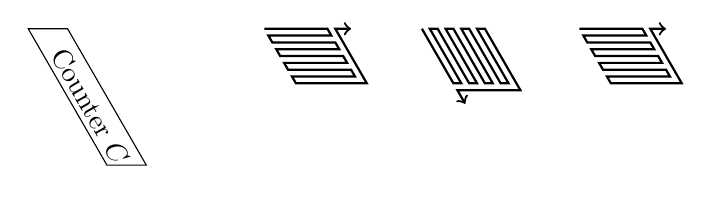
\begin{tikzpicture}

\draw (0, 0) -- ++(0:0.5) -- node[below, sloped] {Counter $C$} ++(300:2) -- ++(180:0.5) -- cycle; 

\foreach \x in {3, 7} {
%\draw (\x, 0) -- ++(0:0.8) -- ++(300:0.8) -- ++(180:0.8) -- cycle;
\draw[thick, ->] (\x, 0) -- ++(0:0.8) -- ++(300:0.1) -- ++(180:0.8) -- ++(300:0.1)
-- ++(0:0.8) -- ++(300:0.1) -- ++(180:0.8) -- ++(300:0.1)
-- ++(0:0.8) -- ++(300:0.1) -- ++(180:0.8) -- ++(300:0.1)
-- ++(0:0.8) -- ++(300:0.1) -- ++(180:0.8) -- ++(300:0.1)
-- ++(0:0.9) -- ++(120:0.8) -- ++(0:0.2)
;
}

\foreach \x in {5} {

\draw[thick, ->] (\x, 0) 
-- ++(300:0.8) -- ++(0:0.1) -- ++(120:0.8) -- ++(0:0.1)
-- ++(300:0.8) -- ++(0:0.1) -- ++(120:0.8) -- ++(0:0.1)
-- ++(300:0.8) -- ++(0:0.1) -- ++(120:0.8) -- ++(0:0.1)
-- ++(300:0.8) -- ++(0:0.1) -- ++(120:0.8) -- ++(0:0.1)
-- ++(300:0.9) -- ++(180:0.8) -- ++(300:0.2)
;
}

\end{tikzpicture}
\caption{Module automaton}
\label{fig:module_automaton}
\end{figure}

%--------------------------------------------------------------------------------------------------------
	\section{Transcript}
%--------------------------------------------------------------------------------------------------------


\end{document}
